% chapters/03_dm_verity.tex
\chapter{dm-verity 完整性校验详细设计}

\section{概述}

dm-verity 实现为块设备提供透明的完整性校验。它通过将读取的数据与预计算的默克尔树（Merkle Tree）进行比对，确保从底层存储层读取的数据未被篡改。该实现强制执行只读策略，以在设备的整个生命周期内维持完整性保证。

在星绽操作系统环境中，dm-verity 主要用于保护根文件系统（rootfs）和关键系统镜像，防止攻击者通过离线篡改持久化存储介质植入后门或破坏系统完整性。

\section{架构组成}

完整性校验系统由三个主要组件构成，下图展示了这些组件的映射关系：

\begin{figure}[H]
    \centering
    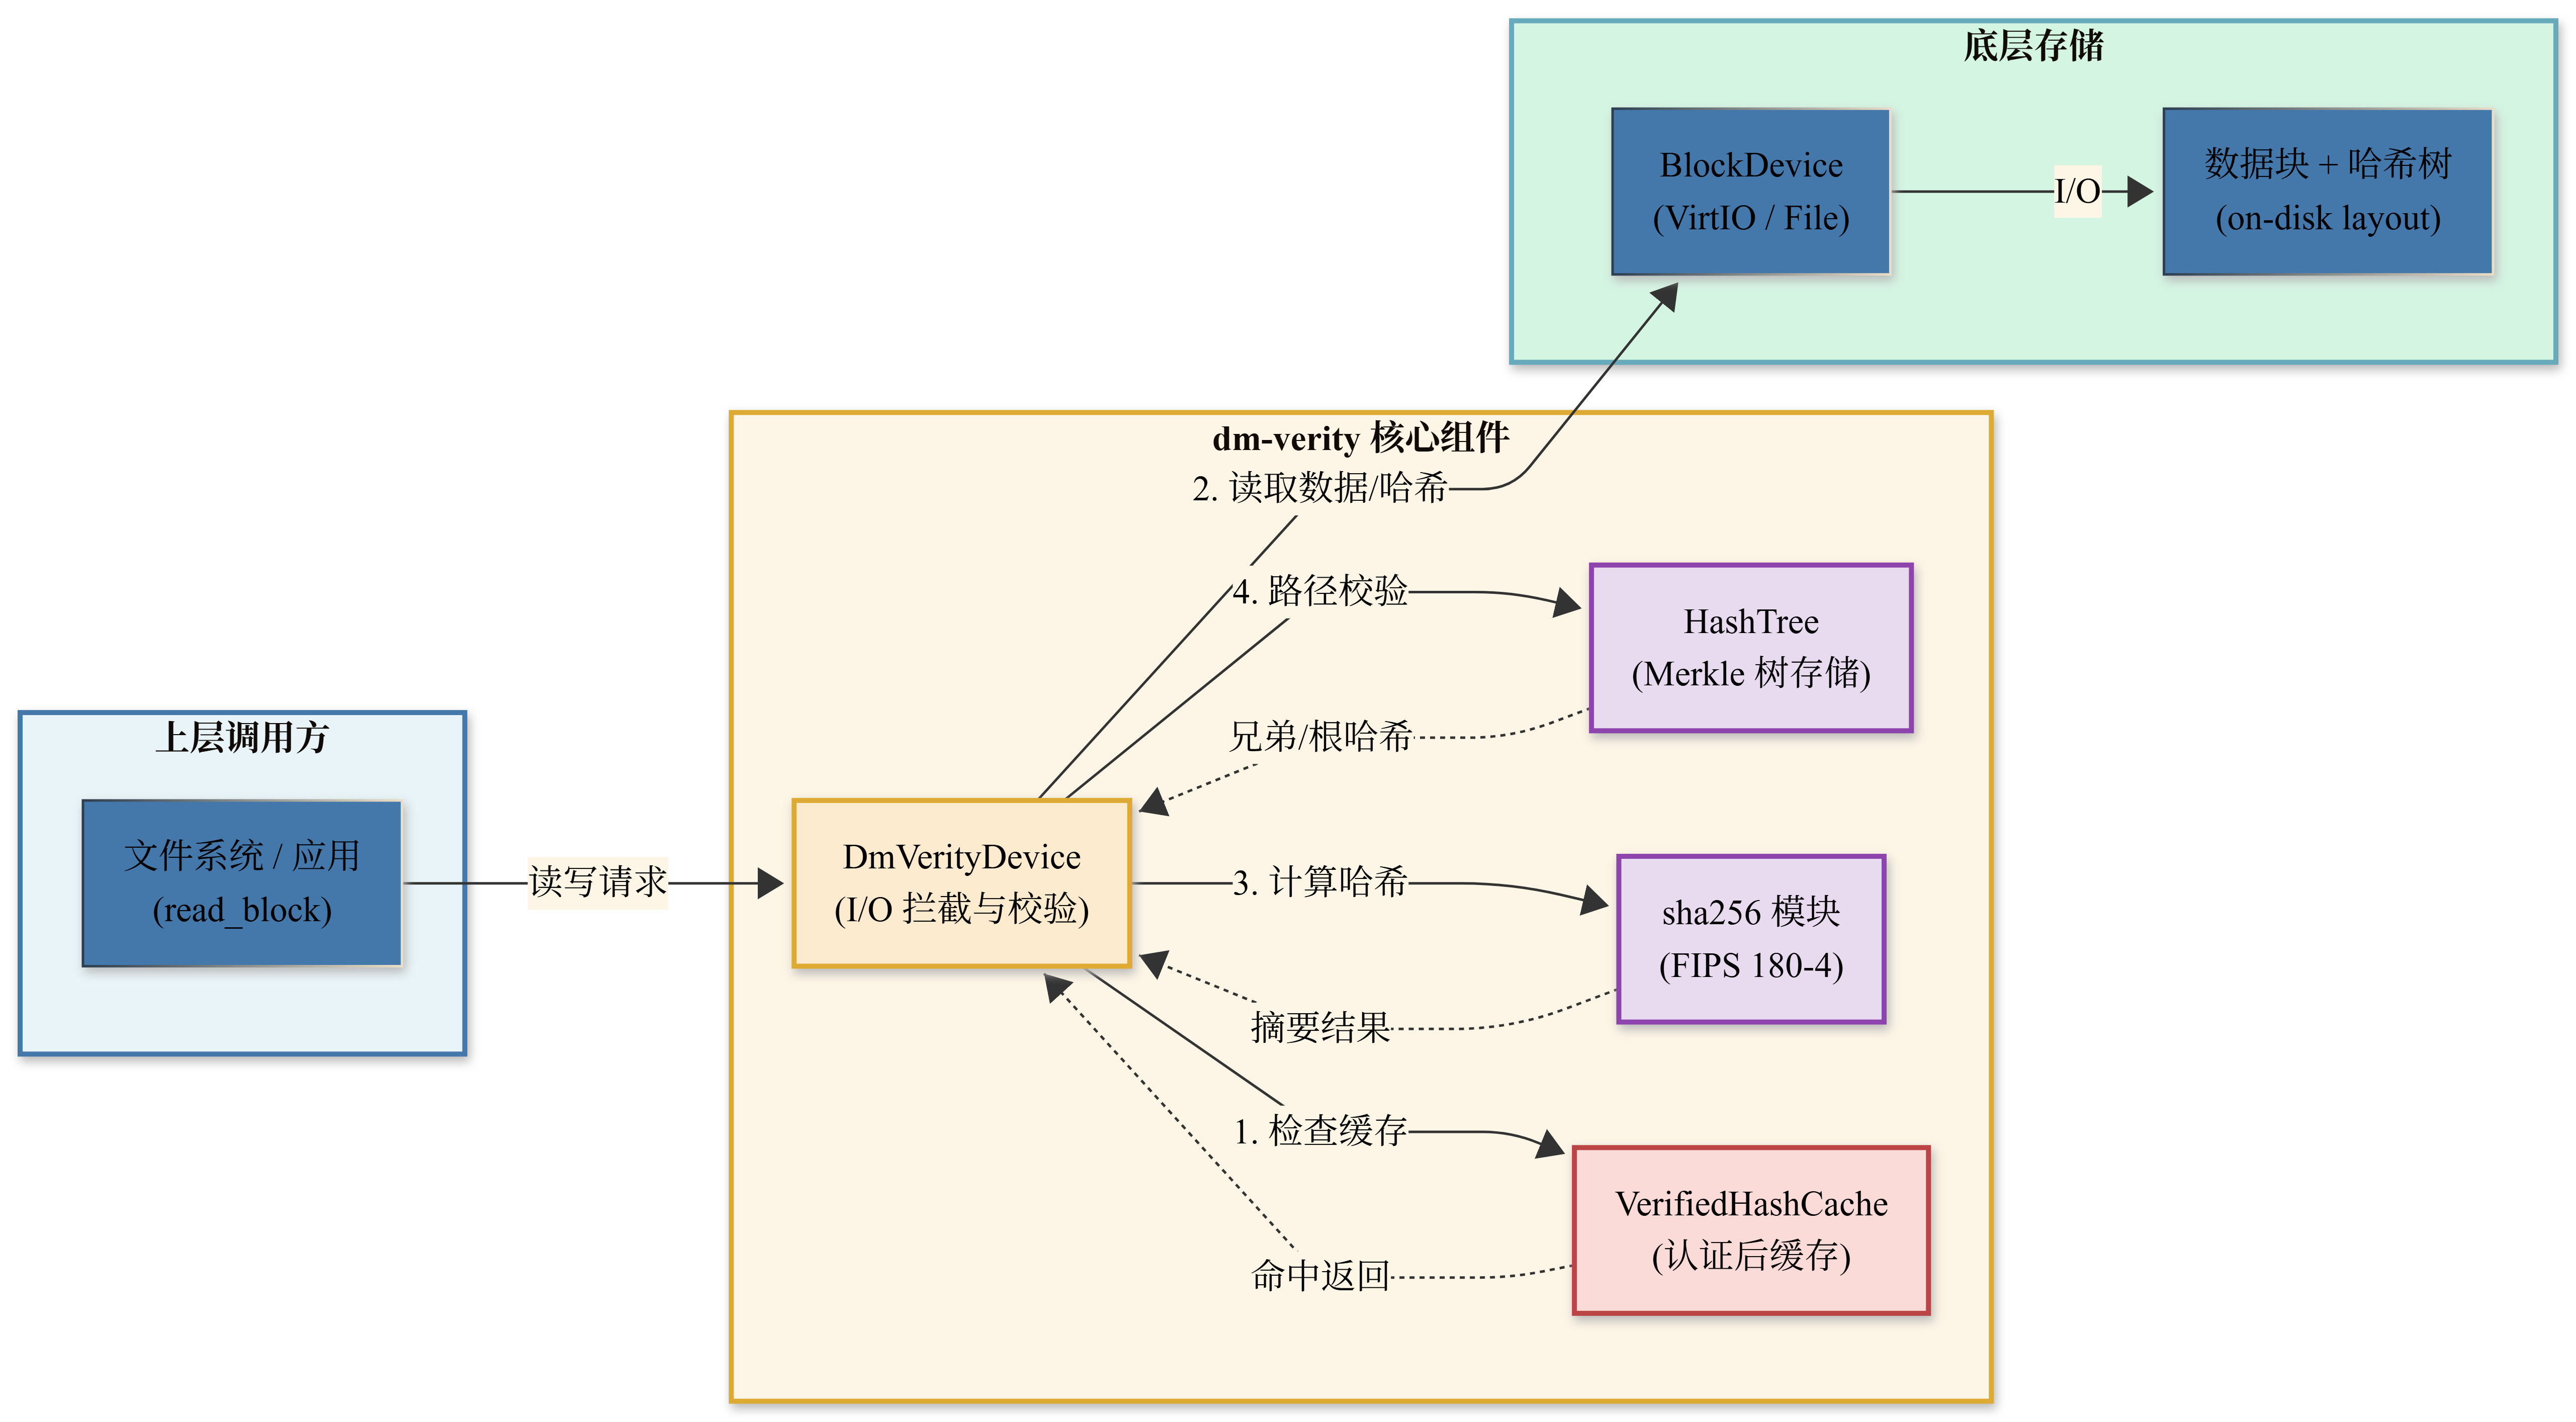
\includegraphics[width=0.85\textwidth]{figures/verity_component_map.png}
    \caption{完整性校验组件映射图}
    \label{fig:verity_components}
\end{figure}

三个核心组件的职责如下：

\begin{itemize}
    \item DmVerityDevice：顶层的 BlockDevice 实现，负责拦截读请求并执行校验操作。它是 dm-verity 对外的接口，所有 I/O 请求首先经过该设备。
    \item HashTree：默克尔树结构，用于存储所有数据块和中间节点的 SHA-256 哈希值。该树在镜像构建时生成，在运行时作为校验的参考依据。
    \item sha256 模块：纯 Rust 实现的 SHA-256 哈希算法，用于所有密码学校验和的计算。该实现不依赖任何外部库，确保在受限的内核环境中也能正常运行。
\end{itemize}

\section{默克尔树构建机制}

\subsection{构建流程}

HashTree 通过递归地对块对进行哈希运算来构建，直到得出单一的根哈希（Root Hash）。构建流程如下：

\begin{enumerate}
    \item 叶子层（Leaf Level）：使用 sha256 对底层设备的每个数据块进行哈希运算，生成叶子节点的哈希值。
    \item 中间层（Intermediate Levels）：将下一层的哈希值两两拼接并进行哈希运算，从而形成上一层。
    \item 填充（Padding）：如果某一层有奇数个哈希值，则最后一个哈希值会被复制一次以凑成一对，确保每层都能配对。
    \item 根哈希（Root Hash）：该过程持续进行，直到只剩下一个哈希值，该值被指定为 root hash，作为整个卷的"信任锚"。
\end{enumerate}

\begin{figure}[H]
    \centering
    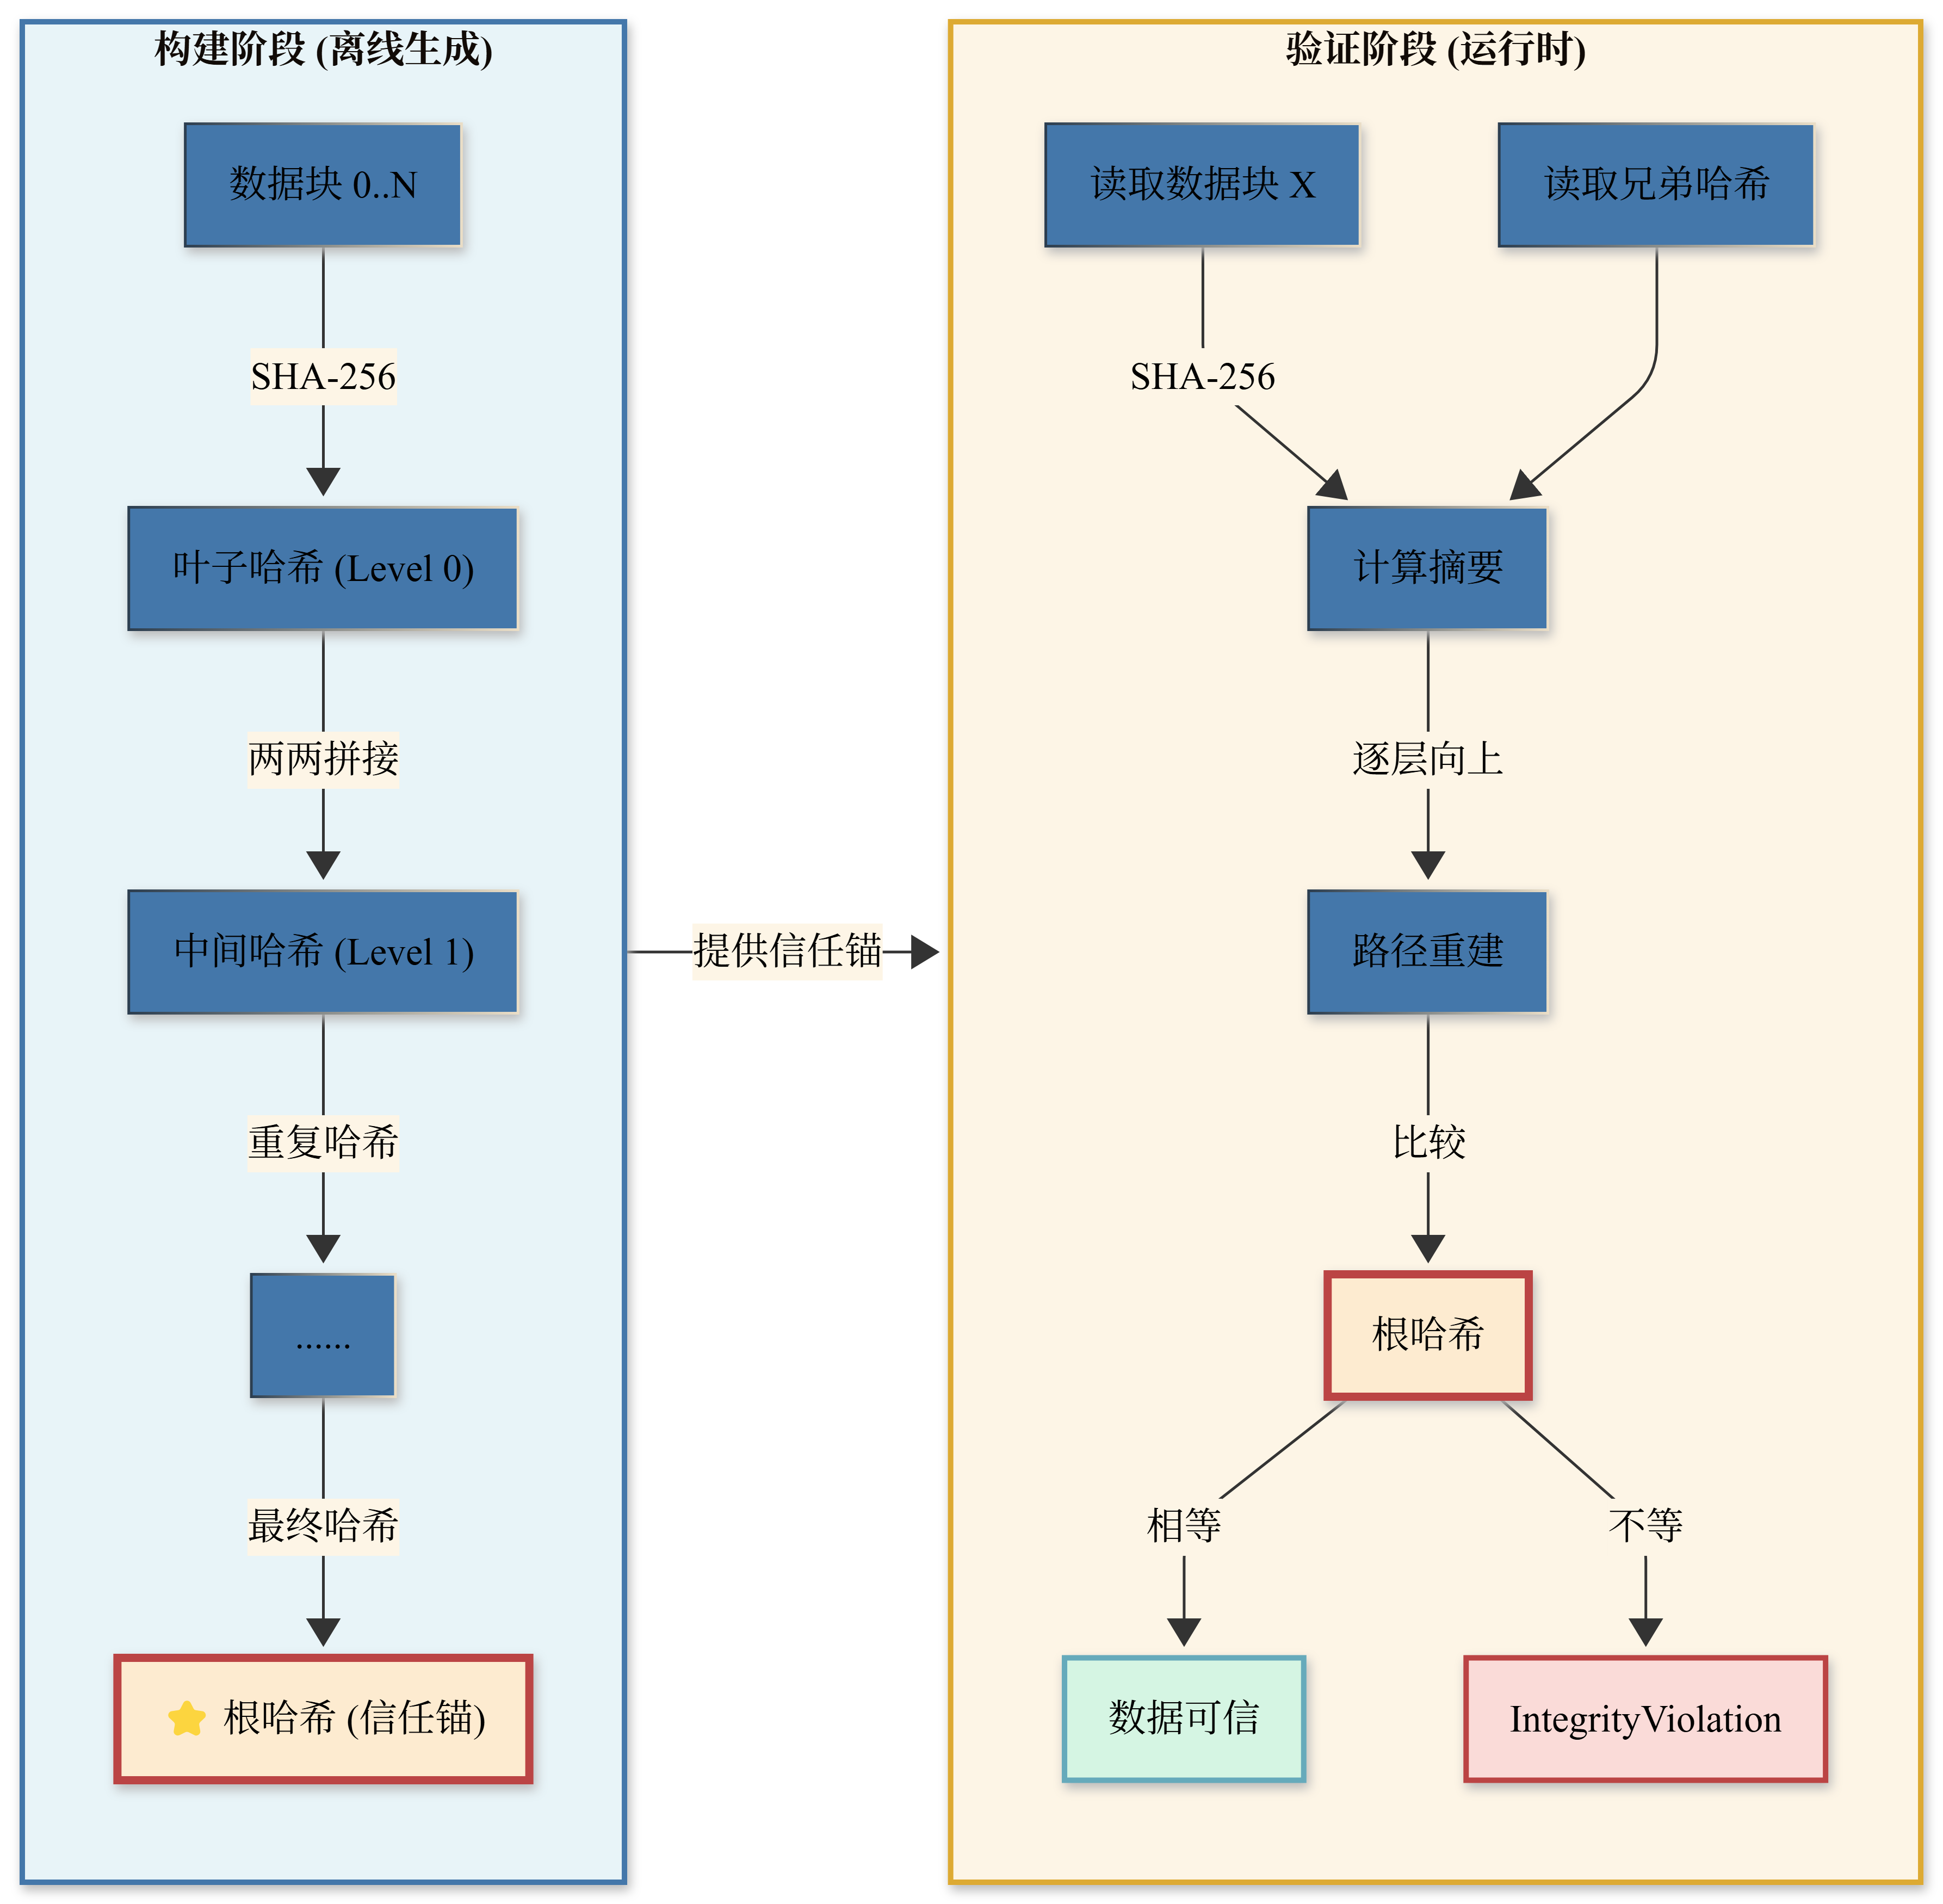
\includegraphics[width=0.9\textwidth]{figures/merkle_tree_flow.png}
    \caption{默克尔树数据流图}
    \label{fig:merkle_tree}
\end{figure}

\subsection{内存与磁盘布局}

默克尔树在内存中以 HashTree 结构体的形式存储，该结构体维护一个层级向量。每一层存储该层所有节点的哈希值（每个节点 32 字节）。

在磁盘布局上，哈希树通常被追加到数据镜像的末尾。这种设计使得标准 ext2 镜像可以与哈希树共存，而无需修改原有的数据布局。构建工具负责将哈希树写入镜像文件，并记录其起始偏移量。

\section{单块校验路径}

当在 DmVerityDevice 上调用 read block 时，会执行以下校验序列：

\begin{enumerate}
    \item 数据检索（Data Retrieval）：从底层块设备读取原始数据块。
    \item 路径校验（Path Verification）：HashTree 的 verify block 函数计算检索到的数据的哈希值，并重新计算其到根节点的路径。
    \item 兄弟节点检索（Sibling Retrieval）：在每一层，从存储的 HashTree 中检索"兄弟"节点的哈希值，用于逐级向上计算。
    \item 根锚点校验（Root Anchor）：将重新计算出的哈希值与 DmVerityDevice 结构体中存储的 root hash 进行比对。
    \item 强制执行（Enforcement）：如果哈希值不匹配，或者树的内部根哈希被篡改，则返回错误，阻止对损坏数据的访问。
\end{enumerate}

\begin{table}[H]
    \centering
    \caption{校验路径关键函数职责}
    \label{tab:verity_functions}
    \begin{tabular}{p{0.35\textwidth}p{0.55\textwidth}}
        \toprule
        \textbf{函数} & \textbf{职责} \\
        \midrule
        DmVerityDevice read block & I/O 的入口点；检查树校验结果与根锚点的比对情况。 \\
        HashTree verify block & 迭代地向上计算树的各层哈希，以校验特定的块 ID。 \\
        sha256 hash & 计算数据块的 32 字节摘要。 \\
        \bottomrule
    \end{tabular}
\end{table}

\section{只读强制策略}

为了确保完整性，DmVerityDevice 明确禁止写操作。任何调用 write block 的尝试都会导致错误。

这种设计反映了 dm-verity 的标准使用场景：哈希树在镜像创建时生成一次，并在运行时仅进行校验。只读策略确保了信任链的完整性，一旦根哈希被验证，整个卷的内容就被锁定，任何写操作都会被拒绝，从而防止攻击者绕过校验机制。

\section{启动参数解析}

为了在系统启动时启用 dm-verity，星绽内核需要从命令行接收配置参数。

\subsection{支持的参数}

\begin{table}[H]
    \centering
    \caption{dm-verity 启动参数}
    \label{tab:verity_boot_params}
    \begin{tabular}{p{0.35\textwidth}p{0.55\textwidth}}
        \toprule
        \textbf{参数} & \textbf{描述} \\
        \midrule
        rootfs verity scheme 等于 dm-verity & 启用 dm-verity 完整性校验标志 \\
        rootfs verity hash & 64 字符十六进制编码的根哈希（32 字节） \\
        \bottomrule
    \end{tabular}
\end{table}

\subsection{解析流程}

解析器按空格分割内核命令行字符串，然后逐个匹配上述键。当检测到 scheme 参数时，启用 verity 标志。当检测到 hash 参数时，将 64 字符的十六进制字符串解码为 32 字节的数组。

解码函数执行严格的长度验证（输入必须恰好 64 个字符），并逐字节解析，任何解析失败都会导致配置无效，从而阻止系统挂载受保护的根文件系统。

\subsection{内核自检机制}

在补丁 0002 中，我们引入了自检机制，用于在启动早期验证 dm-verity 路径的正确性。该机制执行以下操作：

\begin{enumerate}
    \item 通过映射器同步读取第一个块（偏移量 0）。
    \item 检查偏移量 1080（1024 + 56）处的 EXT2 魔数值（0x53EF）。
    \item 如果成功读取到正确的魔数，则证明解密和校验路径功能正常；否则，内核将触发 panic，防止系统在损坏的根文件系统上启动。
\end{enumerate}

\begin{figure}[H]
    \centering
    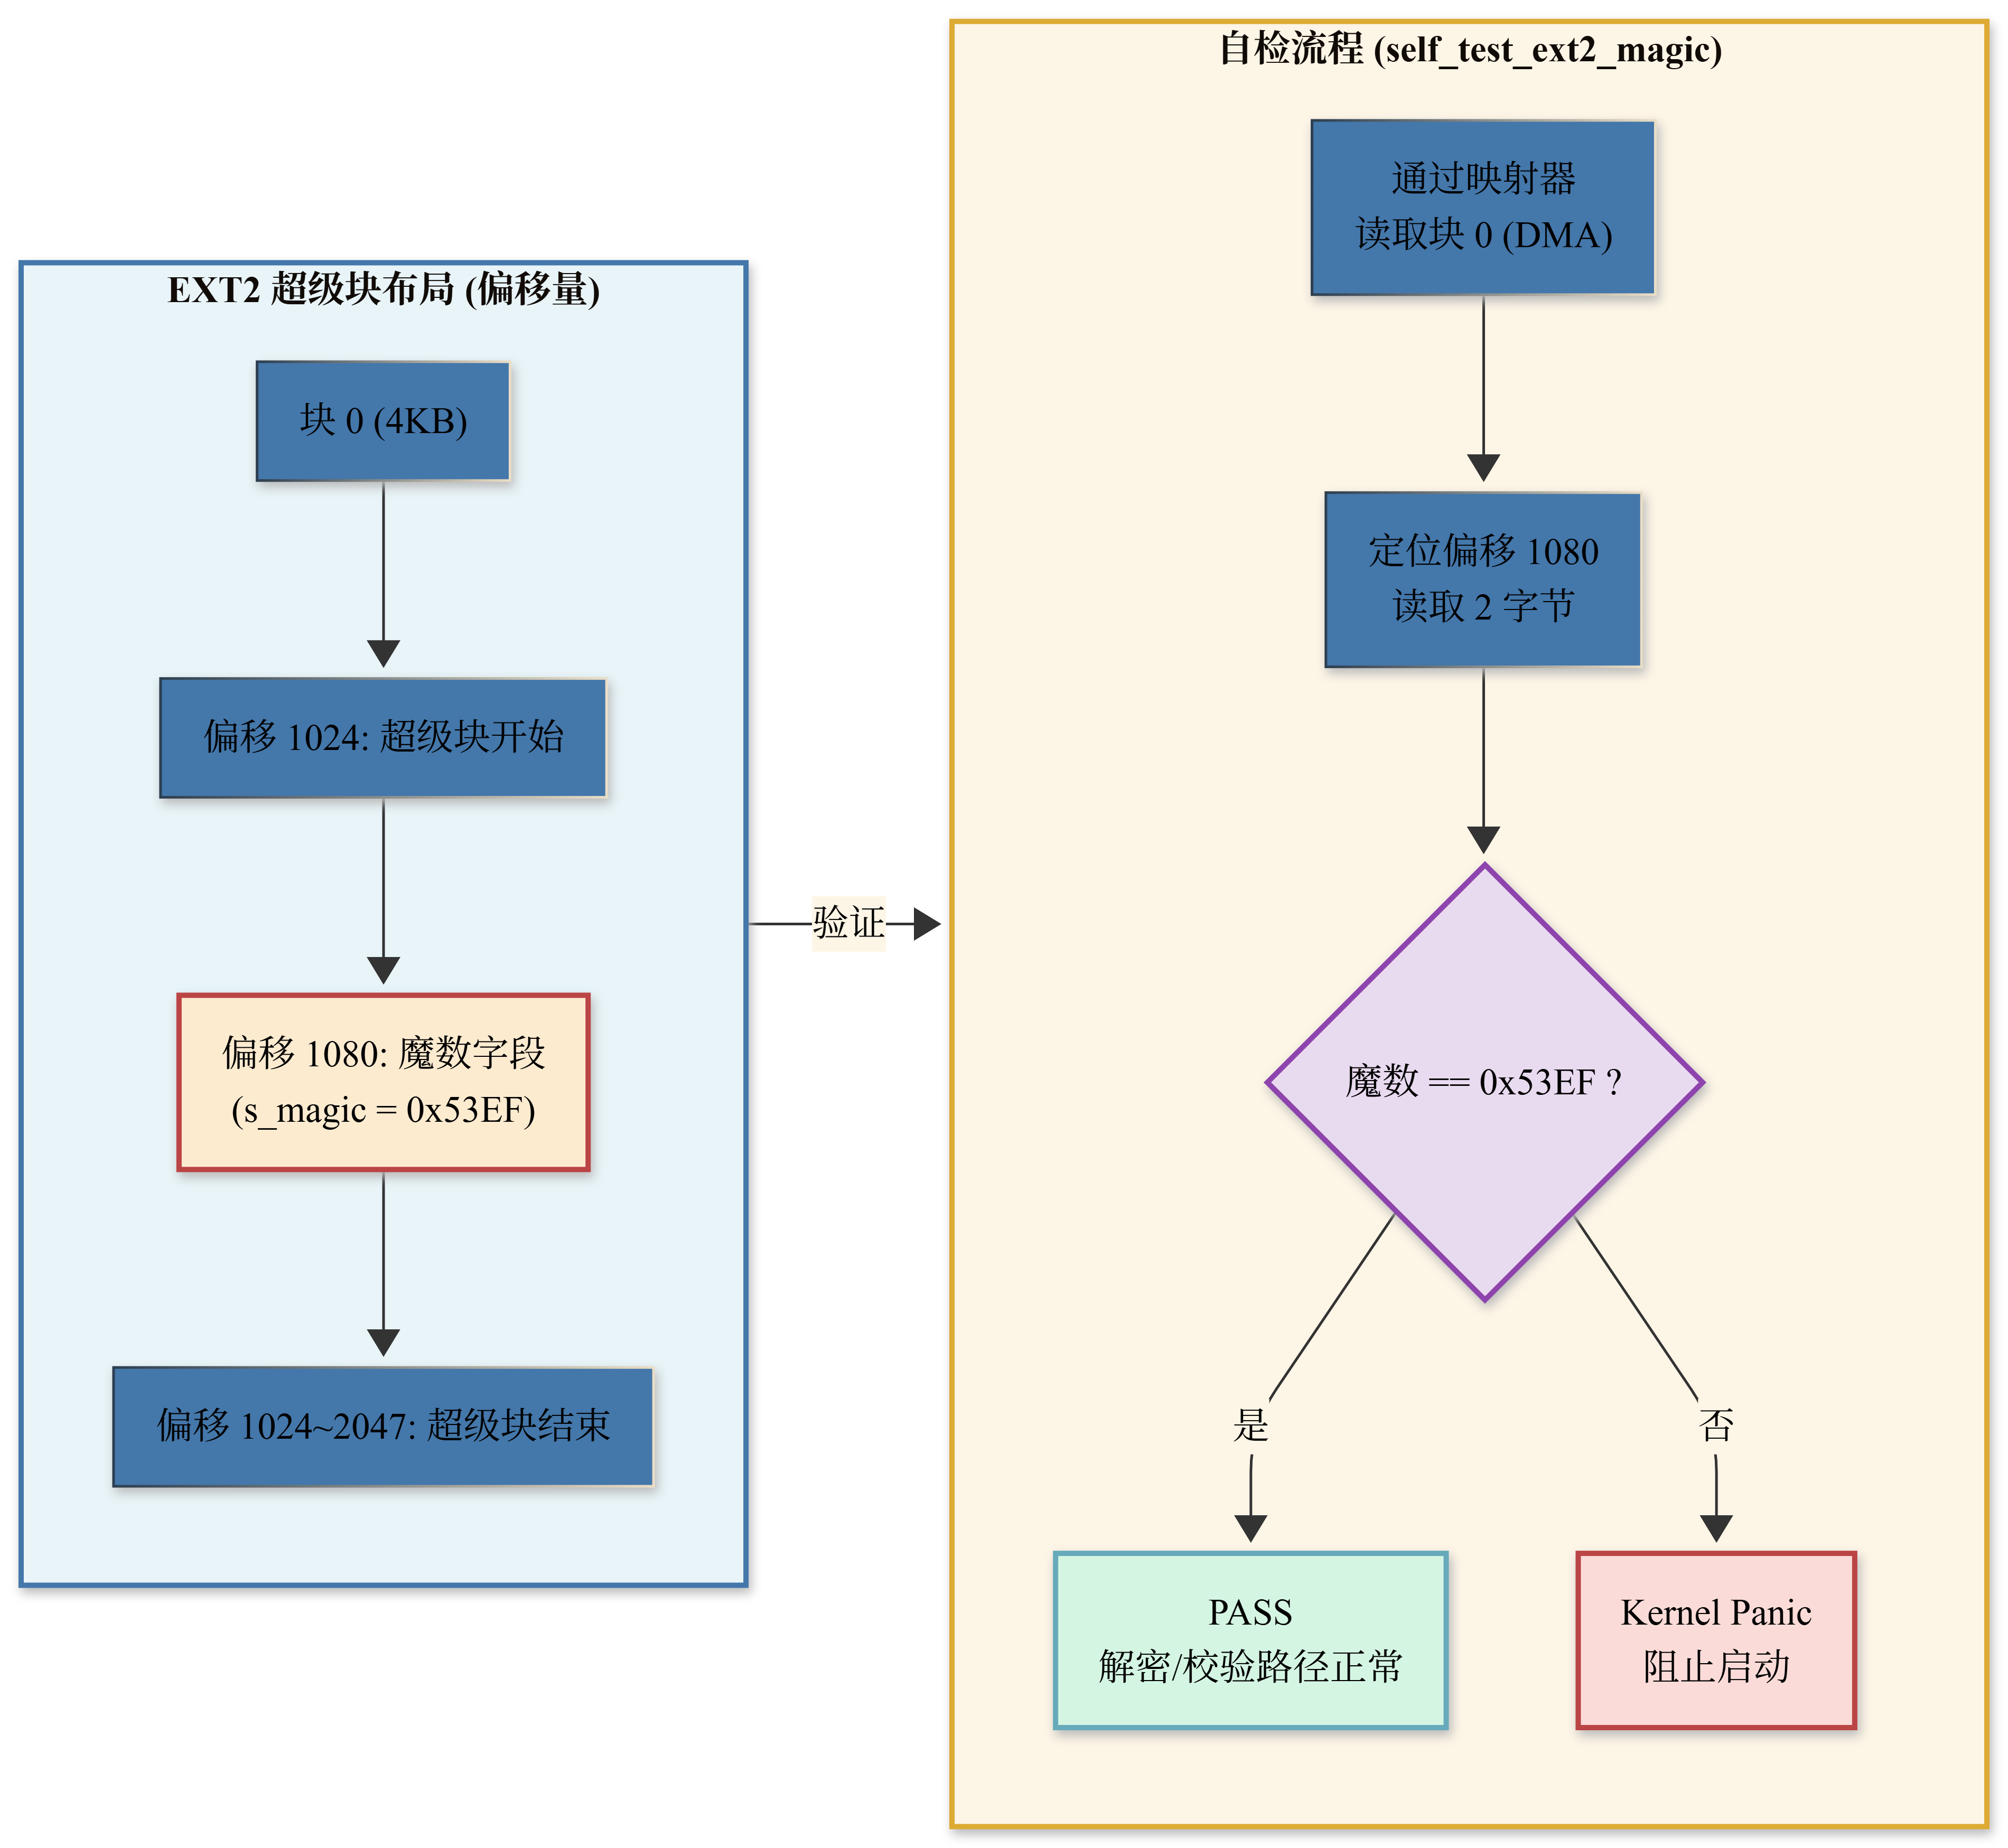
\includegraphics[width=0.85\textwidth]{figures/ext2_superblock_validation.png}
    \caption{Ext2 超级块验证路径图}
    \label{fig:ext2_validation}
\end{figure}

\section{校验失败处理}

当 IntegrityViolation 错误被触发时，系统采取以下措施：

\begin{enumerate}
    \item DmVerityDevice 向调用者返回 I/O 错误。
    \item 如果该错误发生在根文件系统访问期间，内核将触发 panic，阻止系统继续执行任何可能依赖损坏数据的操作。
    \item 如果发生在普通文件访问中，应用程序将收到 I/O 错误，从而可以优雅地处理异常情况。
\end{enumerate}

在篡改检测验证中，我们通过篡改命令在底层镜像中修改单个字节，然后尝试通过 DmVerityDevice 读取该块，确认系统能够正确检测并报告完整性违规。

\section{小结}

本章详细阐述了 dm-verity 的设计与实现，包括默克尔树的构建与校验路径、只读强制策略、启动参数解析以及内核自检机制。通过将哈希树与数据分离存储，并在启动时进行严格的根哈希验证，dm-verity 为星绽操作系统提供了强大的只读完整性保护能力。

在下一章中，我们将转向 dm-crypt 的设计与实现，探讨如何为存储设备提供透明加密保护。